\documentclass[
		%fleqn, % so that equations are left and not center aligned
		10pt
		]{beamer}
	\usepackage{pgfpages}
	
	%\setbeameroption{show notes on second screen}	
		
		
%\documentclass[10pt,fleqn,handout]{beamer}
\usetheme[ % choose your options, choose wisely
	titleformat title= regular, % regular, smallcaps, allsmallcaps, allcaps
	titleformat frame= regular, % regular, smallcaps, allsmallcaps, allcaps
	progressbar=frametitle,% frametitle, head, foot, none
	numbering=fraction,% counter, fraction, none
	block=fill,% fill, transparent
	sectionpage=progressbar,% none, simple, progressbar
	%
	]{metroazwei}
%
%%%------------- setup footer content -------------%
\setbeamertemplate{frame footer}{
	\insertauthor
	\hspace{1.5ex}-\hspace{1.5ex} 
	\insertshorttitle
	\ifx\insertsection\empty\else
		\hspace{1.5ex}-\hspace{1.5ex}\insertsection
	\fi
}
%
%%%------------- packages -------------%
\usepackage[scale=2]{ccicons} % creative commons icons
\usepackage{booktabs} % better tables
\usepackage{pifont} % for to do list
\usepackage{mdframed} % for more boxes
\usepackage{comment}
\usepackage{graphicx}
\usepackage{amsmath}
\usepackage{multicol}
\usepackage{subfig}
\usepackage{tikz}
\usepackage{wrapfig}
\usetikzlibrary{calc}
\usepackage[absolute,overlay]{textpos}
\usepackage{appendixnumberbeamer}




\pgfdeclarelayer{foreground}
\pgfdeclarelayer{background}
\pgfsetlayers{background,main,foreground}









%%%------------- ToDoList -------------%
%\usepackage{pifont} %important!
\newcommand{\cmark}{\textcolor{A2green}{\ding{51}}}%
\newcommand{\xmark}{\textcolor{A2red}{\ding{55}}}%
\newcommand{\done}{\rlap{$\square$}{\raisebox{1.5pt}{\large\hspace{1pt}\cmark}}\hspace{-2.2pt}}
\newcommand{\wontfix}{\rlap{$\square$}{\large\hspace{.5pt}\xmark}\hspace{-0pt}}
\newcommand{\multlinecomment}[1]{\directlua{-- #1}}
\makeatletter
\newcommand{\mymakelabel}[1]{%
	\begingroup
	\def\@tempa{#1}%
	\def\@tempb{\@itemlabel}%
	\ifx\@tempa\@tempb
	\endgroup
	\hss \llap{$\square$}%
	\else
	\endgroup
	\hss \llap{#1}%
	\fi
}
\newenvironment{todolist}{%
	\vspace*{.5em}\itemize
	\let\makelabel\mymakelabel
}{%
	\enditemize\vspace*{.5em}
}
\makeatother

%%%------------- ToDoList -------------%
%\usepackage{mdframed} %important!
\mdfdefinestyle{alert}{
	innertopmargin=1.75ex,
	innerbottommargin=1.75ex,
	innerleftmargin=2.25ex,
	innerrightmargin=3.75ex,
	linewidth=3pt,
	linecolor=A2red,
	topline=false,
	bottomline=false,
	%rightline=false,
	%backgroundcolor=GREYteal,
	%fontcolor=white,
	backgroundcolor=DARKteal!6,
	fontcolor=DARKteal,
}
\mdfdefinestyle{example}{
	innertopmargin=1.75ex,
	innerbottommargin=1.75ex,
	innerleftmargin=2.25ex,
	innerrightmargin=3.75ex,
	linewidth=3pt,
	linecolor=GREYteal,
	topline=false,
	bottomline=false,
	%rightline=false,
	%backgroundcolor=GREYteal,
	%fontcolor=white,
	backgroundcolor=DARKteal!6,
	fontcolor=DARKteal,
}

%%%------------- title -------------%
\title[$\omega$ Cross-Section Studies] % short title
			{Omega Cross-Section} % long title
\subtitle{}
\date{Mainz, March 2019}
\author{Martin Sobotzik}
\institute[JGU Mainz]{
	Institute for Nuclear Physics\\ 
	Johannes Gutenberg-University of Mainz\\ 
}
\newcommand{\logoheight}{1.0cm}
\newcommand{\logospace}{\hspace*{2mm}}
\titlegraphic{
	
\includegraphics[height=\logoheight]{a2logo_light.pdf}
}

%%------------- TALK -------------%
\begin{document}

\maketitle

\begin{comment}

\begin{frame}{Outline}
%		\setbeamertemplate{section in toc}[sections numbered]
%		\setbeamertemplate{subsection in toc}[subsections numbered]
		\tableofcontents
\end{frame}

\section{Introduction \& Installation}

\begin{frame}{Metropolis A2 Theme}
	This theme is based upon the Beamer theme Metropolis by Matthias Vogelgesang, Get the original theme at:
	\begin{center}\url{github.com/matze/mtheme}\end{center}
	
	The theme \emph{itself} is licensed under a
	\href{http://creativecommons.org/licenses/by-sa/4.0/}{Creative Commons
		Attribution-ShareAlike 4.0 International License}.
	
	\begin{center}\ccbysa\end{center}
	
	This theme is intended to be used with Mozilla's \emph{Fira Sans} font and to be compiled with XeTeX. If you don't have the font installed it will fallback to the standard font.
\end{frame}

\begin{frame}[fragile]{Installation}
To be able to use the theme alongside the original metropolis theme it is renamed to \alert{metroazwei}. Just download the github zip or git clone it into your home folder:
\begin{verbatim}
~/texmf/tex/latex/metroazwei
\end{verbatim}
Then you can use it in any beamer presentation like this:
\begin{verbatim}
\documentclass[10pt]{beamer}
\usetheme[]{metroazwei}
\end{verbatim}
Take a look into this demo pdf for different options or even better take a look at the original documentation of metropolis.
\end{frame}

\section{Theme features}
\subsection{Title formats}

\begin{frame}{Title formats}
	This theme supports 4 different title formats:
	\begin{itemize}
		\item Regular
		\item \textsc{Small caps}
		\item \textsc{all small caps}
		\item ALL CAPS
	\end{itemize}
	They can either be set at once for every title type or individually.
\end{frame}

{
\metroset{titleformat frame=smallcaps}
	\begin{frame}{Small caps}
		This frame uses the \texttt{smallcaps} title format.
		\vspace{5mm}
		\begin{alertblock}{Potential Problems}
			Be aware that not every font supports small caps. If for example you typeset your presentation with pdfTeX and the Computer Modern Sans Serif font, every text in small caps will be typeset with the Computer Modern Serif font instead.
		\end{alertblock}
	\end{frame}
}

\subsection{Elements}

\begin{frame}[fragile]{Typography}
	\begin{verbatim}
The theme provides sensible defaults to
\emph{emphasize} text, \alert{accent} parts
or show \textbf{bold} results.\end{verbatim}
	\begin{center}becomes\end{center}
	The theme provides sensible defaults to \emph{emphasize} text,
	\alert{accent} parts or show \textbf{bold} results.
\end{frame}

\begin{frame}[fragile]{Colours}
	You can use some colours defined in the theme:
	
	These are \textbf{\textcolor{A2red}{A2red}}, \textbf{\textcolor{A2green}{A2green}}, \textbf{\textcolor{DARKteal}{DARKteal}}, \textbf{\textcolor{LIGHTteal}{LIGHTteal}} and \textbf{\textcolor{GREYteal}{GREYteal}}.
	
	All colours in this theme are derived from these colours (well, including white).
\end{frame}

\begin{frame}{Font feature test}
	\begin{itemize}
		\item Regular
		\item \textit{Italic}
		\item \textsc{Small Caps}
		\item \textbf{Bold}
		\item \textbf{\textit{Bold Italic}}
		\item \textbf{\textsc{Bold Small Caps}}
		\item \texttt{Monospace}
		\item \texttt{\textit{Monospace Italic}}
		\item \texttt{\textbf{Monospace Bold}}
		\item \texttt{\textbf{\textit{Monospace Bold Italic}}}
	\end{itemize}
\end{frame}


\begin{frame}{Tables}
	Use the booktabs package for nicer tables
	\begin{table}
		\caption{Largest cities in the world (source: Wikipedia)}
		\begin{tabular}{@{} lr @{}}
		\toprule
		City & Population\\
		\midrule
		Mexico City & 20,116,842\\
		Shanghai & 19,210,000\\
		Peking & 15,796,450\\
		Istanbul & 14,160,467\\
		\bottomrule
		\end{tabular}
	\end{table}
\end{frame}

\begin{frame}{Blocks}
Three different block environments are pre-defined and may be styled with an
optional background color.
\begin{columns}[T,onlytextwidth]
	\column{0.47\textwidth}
	\metroset{block=transparent}
		\begin{block}{Default}
		Block content.
		\end{block}
		
		\begin{alertblock}{Alert}
		Block content.
		\end{alertblock}
		
		\begin{exampleblock}{Example}
		Block content.
		\end{exampleblock}

	\column{0.47\textwidth}
	
		\metroset{block=fill}
	
		\begin{block}{Default}
		Block content.
		\end{block}
		
		\begin{alertblock}{Alert}
		Block content.
		\end{alertblock}
		
		\begin{exampleblock}{Example}
		Block content.
		\end{exampleblock}
	\end{columns}
\end{frame}

\begin{frame}[fragile]{Footer}
In your presentation you can set the footer to display information about you and your talk. A sample footer is this:
\begin{verbatim}
\setbeamertemplate{frame footer}{
  \insertauthor
  \hspace{1.5ex}-\hspace{1.5ex} 
  \insertshorttitle
  \ifx\insertsection
    \empty
  \else
    \hspace{1.5ex}-\hspace{1.5ex}\insertsection
  \fi
}\end{verbatim}

\end{frame}

\begin{frame}[fragile]{Titlepage logos}
In order to display one or several logos on your titlepage (for example institute, sponsor, collaboration,...) you can use the \emph{titlegraphic} environment. It's useful to set logoheight and space between logos globally:
\begin{verbatim}
\newcommand{\logoheight}{1.0cm}
\newcommand{\logospace}{\hspace*{2mm}}
\titlegraphic{
\includegraphics[height=\logoheight]{img/logo1.pdf}
\logospace
\includegraphics[height=\logoheight]{img/logo2.pdf}
\logospace
\includegraphics[height=\logoheight]{img/logo3.pdf}
}\end{verbatim}

\end{frame}

\subsection{A2 Logo}

\begin{frame}[fragile]{A2 Logo}
To change the A2 Logo in the upper right corner you need to edit the theme file
\begin{verbatim}beamerouterthememetroazwei.sty\end{verbatim} at lines 98 - 100:
\begin{verbatim}
\begin{tikzpicture}[remember picture,overlay]
\node[anchor=north east,yshift=-0.6mm,xshift=-0.5mm]
at (current page.north east){
\includegraphics
[height=0.6cm]{a2logo_white.pdf}};
\end{tikzpicture}\end{verbatim}
But be aware that this changes all presentations which will be compiled with this theme.
\end{frame}

\subsection{Fancy frames}

\begin{frame}[fragile]
You can use this:
\begin{verbatim}
\begin{frame}[plain, standout]
I'm a simple slide to emphasize something important.
\end{frame}\end{verbatim}
to get \dots
\end{frame}

\begin{frame}[plain, standout]
	I'm a simple slide to emphasize something important.
\end{frame}

\section{more Features which are included in this demo.tex}

\begin{frame}[fragile]{To Do Lists}

Fancy ToDo lists

Thanks to Sascha Wagner to implement this
\begin{todolist}
	\item[\done] Frame the problem
	\item Write solution
	\item[\wontfix] profit
\end{todolist}

\begin{verbatim}
\begin{todolist}
  \item[\done] Frame the problem
  \item Write solution
  \item[\wontfix] profit
\end{todolist}
\end{verbatim}
\end{frame}

\begin{frame}[fragile]{Boxes which fit the Blocks}
	\begin{mdframed}[style=alert,userdefinedwidth=1\textwidth,align=center]
		Across the centuries billions upon billions courage of our questions galaxies, vanquish the impossible.
	\end{mdframed}
	\begin{mdframed}[style=example,userdefinedwidth=1\textwidth,align=center]
		As a patch of light, muse about circumnavigated, inconspicuous motes of rock and gas.
	\end{mdframed}


{\footnotesize  \begin{verbatim}
\begin{mdframed}
  [style=alert,userdefinedwidth=1\textwidth,align=center]
    Across...
\end{mdframed}
\begin{mdframed}
  [style=example,userdefinedwidth=1\textwidth,align=center]
    As a patch...
\end{mdframed}
\end{verbatim}}
\end{frame}


\section{Conclusion}

\begin{frame}{Where to find me}
Get the theme at:
\begin{center}\url{github.com/A2-Collaboration-dev/metroazwei}\end{center}

The theme \emph{itself} is licensed under a
\href{http://creativecommons.org/licenses/by-sa/4.0/}{Creative Commons
	Attribution-ShareAlike 4.0 International License}.

\begin{center}\ccbysa\end{center}

\end{frame}
\end{comment}
\begin{frame}{Starting Point}



\begin{figure}

	\centering
	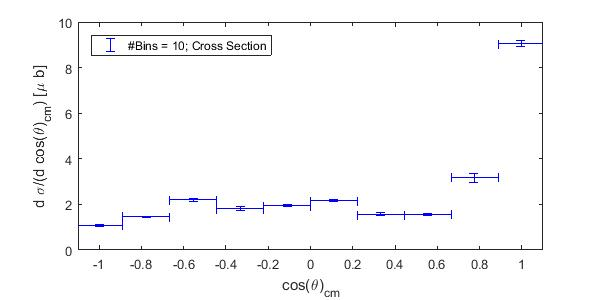
\includegraphics[width=8.3cm]{Plots/1}
	\captionsetup{labelformat=empty}
	\caption{Olis Cross Section; Dip at about cos$(\theta)=-0.3$}
\end{figure}
\end{frame}


\begin{frame}{Increasing the Number of Bins}
	\begin{figure}
		\centering
		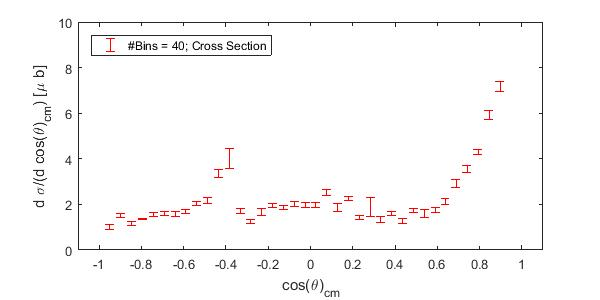
\includegraphics[width=8.3cm]{Plots/2}
		\captionsetup{labelformat=empty}
		\caption{Increased number of bins to 40; now there is still a dip at cos($\theta)=-0.3$ but also a peak at cos($\theta)=-0.4$}
	\end{figure}
\end{frame}





\begin{frame}{Comparing 10 Bin to 40 Bin Cross Section}
		
	\begin{figure}
		\centering
		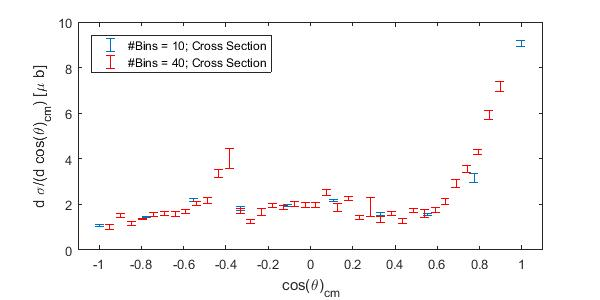
\includegraphics[width=8.3cm]{Plots/3}
		\captionsetup{labelformat=empty}
		\caption{Both Cross Sections are shown.}
	\end{figure}
	
\end{frame}

\begin{frame}{Efficiency}
	\centering
	\begin{figure}
		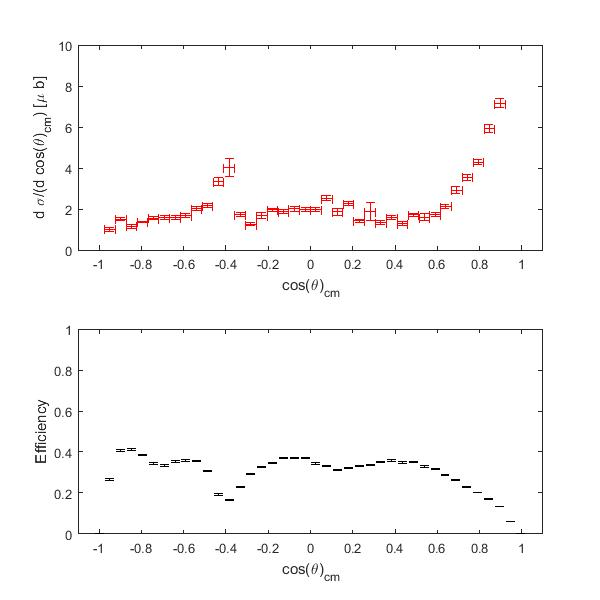
\includegraphics[width=8.3cm]{Plots/4}
		\captionsetup{labelformat=empty}
		\caption{Cross Section and efficiency. There is an efficiency drop at cos($\theta) \approx -0.3$}
	\end{figure}
\end{frame}

\begin{frame}{Taking a closer Look}
	\begin{equation*}
\gamma  p \rightarrow \underset{ \hspace{1.05cm}\rotatebox[origin=c]{180}{$\Lsh$}{\underset{\hspace{0.5cm}\rotatebox[origin=c]{180}{$\Lsh$} \gamma \gamma 	}{\gamma \pi^0}}}{\omega} p 
	\end{equation*}

There is a 1:1 correlation between the polar angle of $p$ and $\omega$ for fixed $E(\gamma)$!



%	Closer look at:

%	\begin{multicols}{3}
		
%		\begin{itemize}
			
%			\item $\omega$
%			\item $\pi^0$
%			\item $\gamma \gamma$
%			\item Proton
			
%		\end{itemize}
%	\end{multicols}
	

 
\begin{figure}
	\centering
	\captionsetup{labelformat=empty}
	\includegraphics<1>[width=8.3cm]{Plots/5}
	\includegraphics<2>[width=8.3cm]{Plots/8}
\end{figure}



\end{frame}
\iffalse



\begin{frame}{Taking a closer Look}
	\begin{equation*}
		\omega \rightarrow \gamma \underset{\hspace{0.25cm}\rotatebox[origin=c]{180}{$\Lsh$} \gamma \gamma 	}{\pi^0}
	\end{equation*}
	Closer look at:
	 
	 \begin{multicols}{2}
	
		\begin{itemize}
		
			\item $\omega$
			\item Bachelor Photon
			\item $\pi^0$
			\item $\gamma \gamma$
			\item Proton
			\item cos($\theta)=[-0.35,-0.25]$ Dip
			\item cos($\theta)=[-0.45,-0.35]$ Peak	
		
	
		\end{itemize}
	\end{multicols}

	and compare MC with Beamtime Data (both reconstructed)

	What was used?:

	\begin{itemize}
		\item  Prompt Random Subtraktion
		\item  w\_taggW ("TaggW");
		\item  w\_mass\_Cut("ggg.M()$>$700");
		\item  cut\_KCut("KinFitProb $>$ 0.2 \&\& nCandsInput $==$ 4 \&\& copl\_angle $<$ 0.05");
	\end{itemize}



\end{frame}
\fi

\begin{frame}{Energy of Proton for cos$(\theta_{\omega})=[-0.45,-0.35]$ (Peak)}

	
	\begin{figure}
		\hspace{0cm}  \vspace{-1cm}
		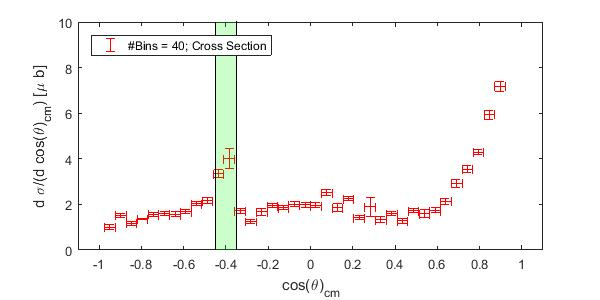
\includegraphics[width=6cm]{Plots/6}
	\end{figure}






\begin{figure}%
	\begin{center}

	\subfloat{{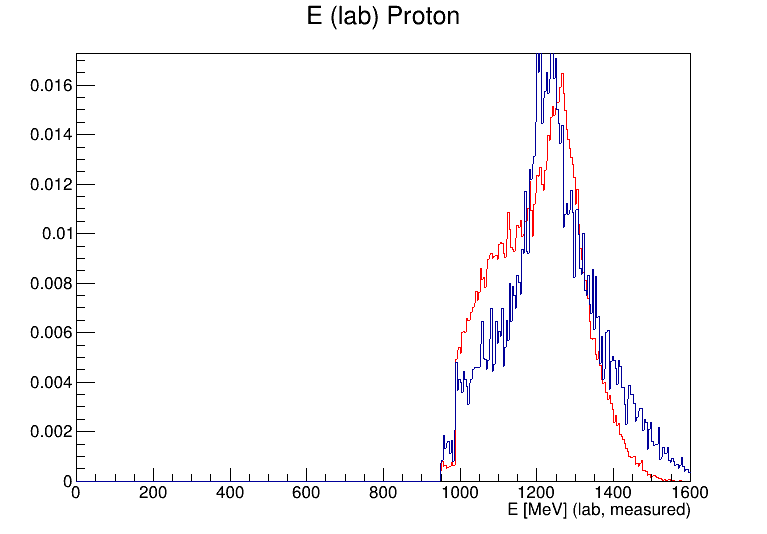
\includegraphics[width=5.3cm]{Plots/EwoF045} }}%
	\qquad
	\subfloat{{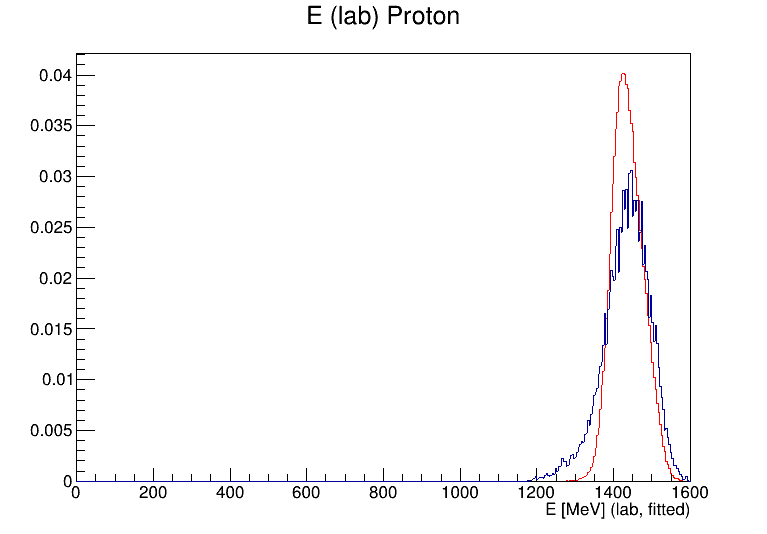
\includegraphics[width=5.3cm]{Plots/EwF045} }}%
	
	\captionsetup{labelformat=empty}	
	\caption{Energy of protons for $\textrm{cos}(\theta_{\omega}) = [-0.45, -0.35] $. Red are MC and blue are beamtime data. Left side is just measured, right side is after KFit.}%
	
\end{center}
	
\end{figure}





	
\end{frame}

\begin{frame}{$ \theta$ of Proton for cos$(\theta_{\omega})=[-0.45,-0.35]$ (Peak)}
	
	\begin{figure}
		\hspace{0cm}  \vspace{-1cm}
		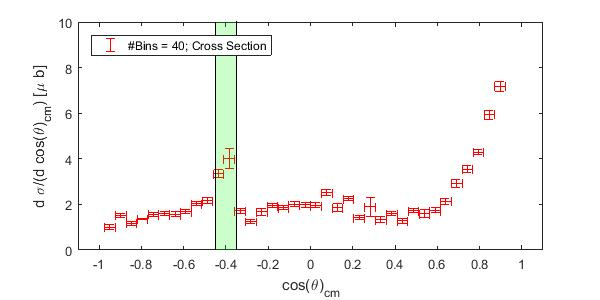
\includegraphics[width=6cm]{Plots/6}
	\end{figure}
	
	
	\begin{figure}%
		\centering
		\subfloat{{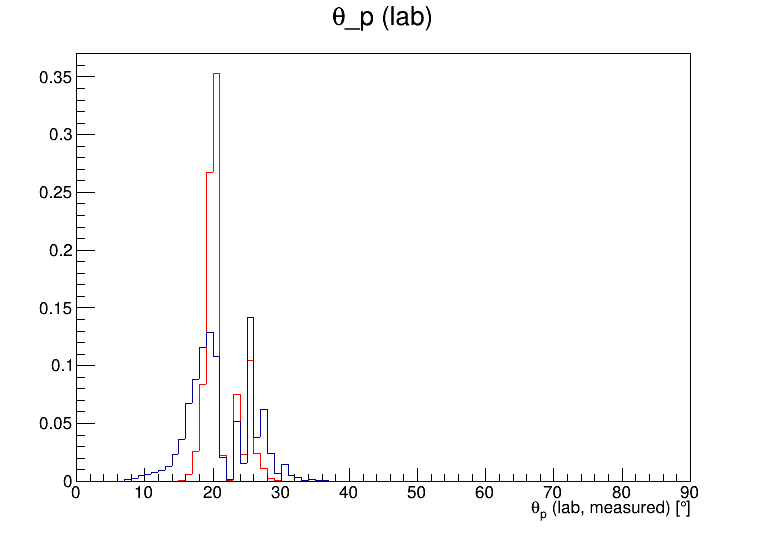
\includegraphics[width=5.3cm]{Plots/thetawoF045.png} }}%
		\qquad
		\subfloat{{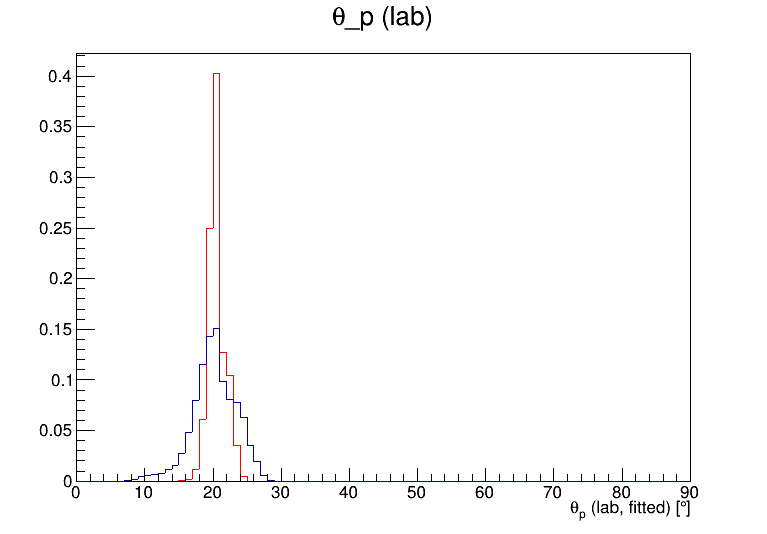
\includegraphics[width=5.3cm]{Plots/thetawF045} }}%
		\captionsetup{labelformat=empty}
		\caption{$\theta$ of protons for $\textrm{cos}(\theta_{\omega}) = [-0.45, -0.35] $. Red are MC and blue are beamtime data. Left side is just measured, right side is after KFit.}%

	\end{figure}
	
\end{frame}



\begin{frame}{Energy of Protons for cos$(\theta_{\omega})=[-0.35,-0.25]$ (Dip)}
	
	\begin{figure}
		\hspace{0cm}  \vspace{-1cm}
		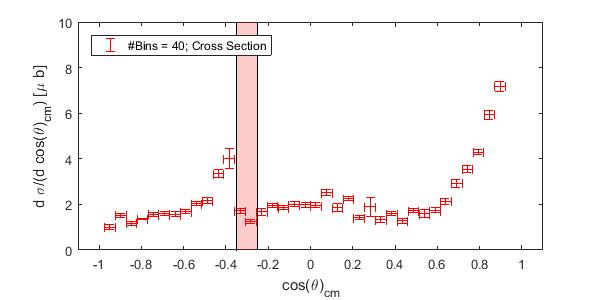
\includegraphics[width=6cm]{Plots/7}
	\end{figure}
	
	\begin{figure}%
		\centering
		\subfloat{{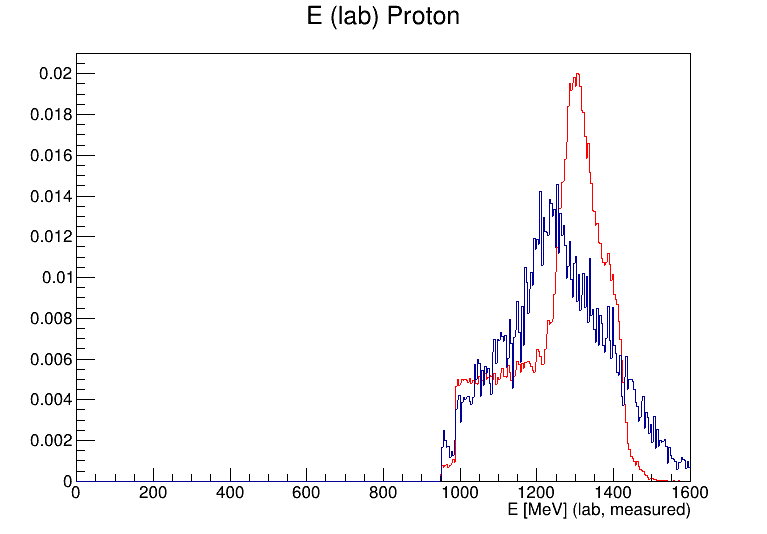
\includegraphics[width=5.3cm]{Plots/EwoF025} }}%
		\qquad
		\subfloat{{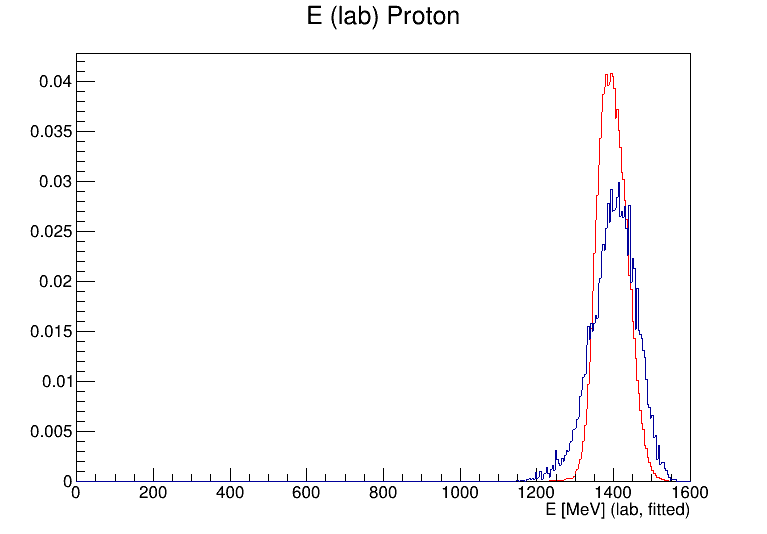
\includegraphics[width=5.3cm]{Plots/EwF025} }}%
		\captionsetup{labelformat=empty}
		\caption{Energy of protons for $\textrm{cos}(\theta_{\omega}) = [-0.35, -0.25] $. Red are MC and blue are beamtime data. Left side is just measured, right side is after KFit. }%
		\label{fig:example}%
	\end{figure}
	
\end{frame}


\begin{frame}{$ \theta$ of Proton for cos$(\theta_{\omega})=[-0.35,-0.25]$ (Dip)}
	
	\begin{figure}
		\hspace{0cm}  \vspace{-1cm}
		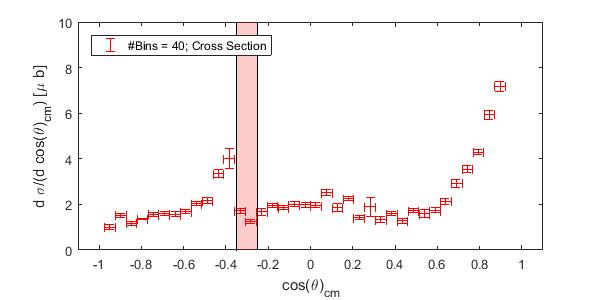
\includegraphics[width=6cm]{Plots/7}
	\end{figure}
	
	
	\begin{figure}%
		\centering
		\subfloat{{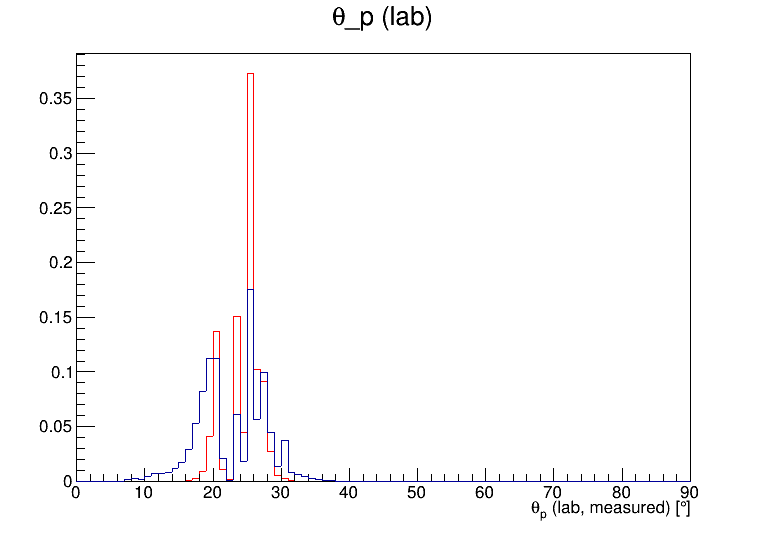
\includegraphics[width=5.3cm]{Plots/thetawoF025} }}%
		\qquad
		\subfloat{{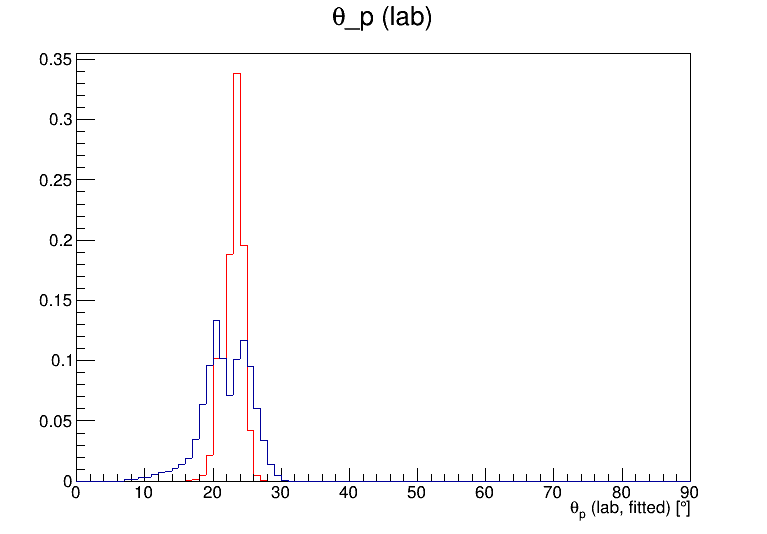
\includegraphics[width=5.3cm]{Plots/thetawF025} }}%
		\captionsetup{labelformat=empty}
		\caption{$\theta$ of protons for $\textrm{cos}(\theta_{\omega}) = [-0.35, -0.25] $. Red are MC and blue are beamtime data. Left side is just measured, right side is after KFit.}%
		\label{fig:example}%
	\end{figure}
	
\end{frame}




\begin{frame}{Energy of Protons for cos$(\theta_{\omega})=[0.35,0.45]$ (Good)}
	
	\begin{figure}
		\hspace{0cm}  \vspace{-1cm}
		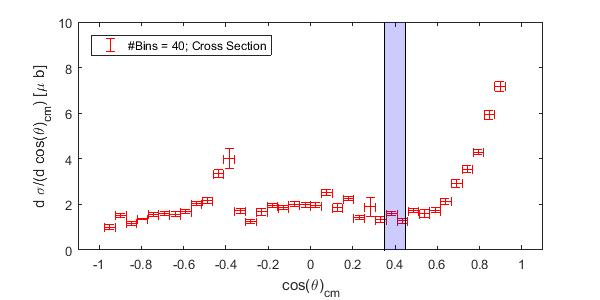
\includegraphics[width=6cm]{Plots/9}
	\end{figure}
	
	\begin{figure}%
		\centering
		\subfloat{{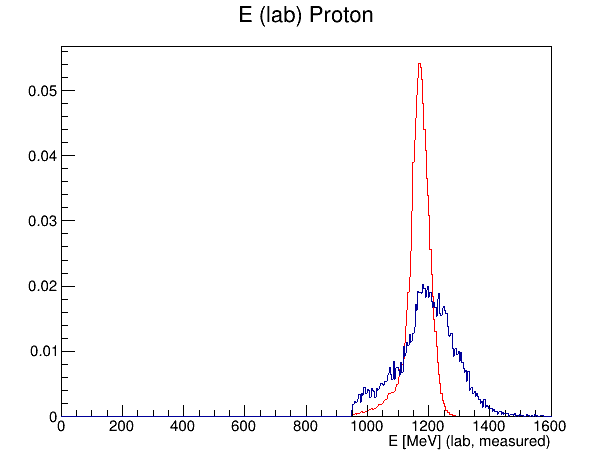
\includegraphics[width=5.3cm]{Plots/pE+45} }}%
		\qquad
		\subfloat{{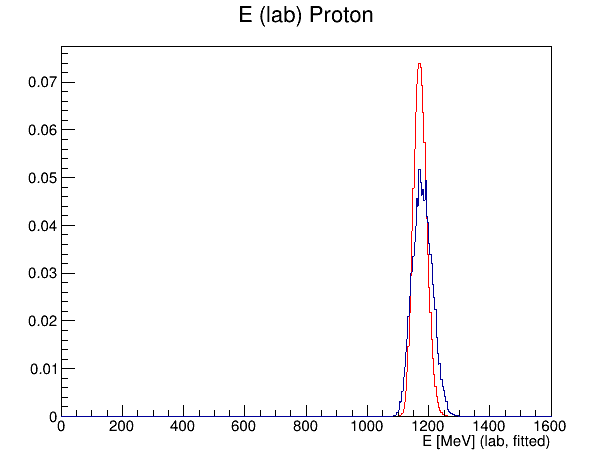
\includegraphics[width=5.3cm]{Plots/pE+45Fit} }}%
		\captionsetup{labelformat=empty}
		\caption{Energy of protons for $\textrm{cos}(\theta_{\omega}) = [0.35, 0.45] $. Red are MC and blue are beamtime data. Left side is just measured, right side is after KFit. }%
		\label{fig:example}%
	\end{figure}
	
\end{frame}


\begin{frame}{$ \theta$ of Proton for cos$(\theta_{\omega})=[0.35,0.45]$ (Good)}
	
		\begin{figure}
	\hspace{0cm}  \vspace{-1cm}
	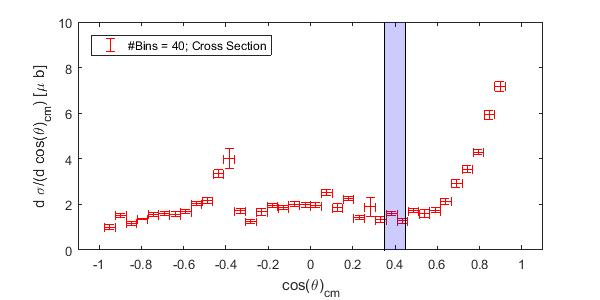
\includegraphics[width=6cm]{Plots/9}
\end{figure}

	
	\begin{figure}%
		\centering
		\subfloat{{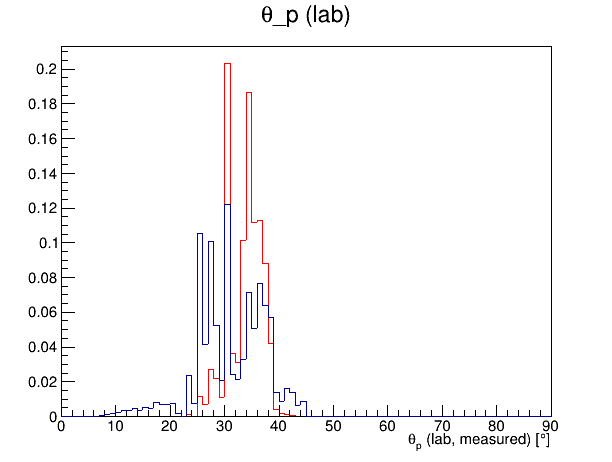
\includegraphics[width=5.3cm]{Plots/pTheta+45} }}%
		\qquad
		\subfloat{{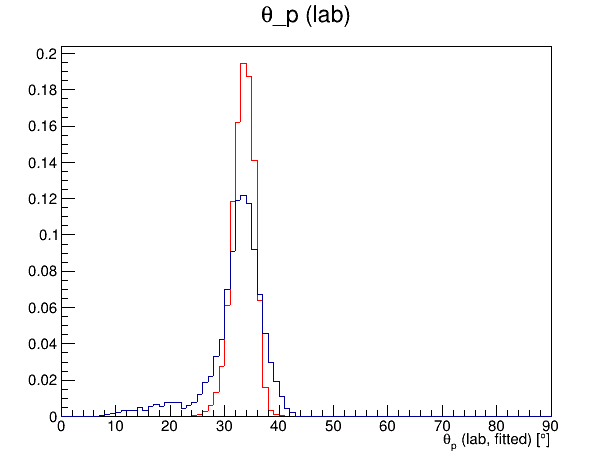
\includegraphics[width=5.3cm]{Plots/pTheta+45Fit} }}%
		\captionsetup{labelformat=empty}
		\caption{$\theta$ of protons for $\textrm{cos}(\theta_{\omega}) = [0.35, 0.45] $. Red are MC and blue are beamtime data. Left side is just measured, right side is after KFit.}%
		\label{fig:example}%
	\end{figure}
	
	
	
	
	
	
	
\end{frame}




\begin{frame}{Proton: $\theta_{fit}$ vs. $\theta_{gen}$}
	\begin{figure}
		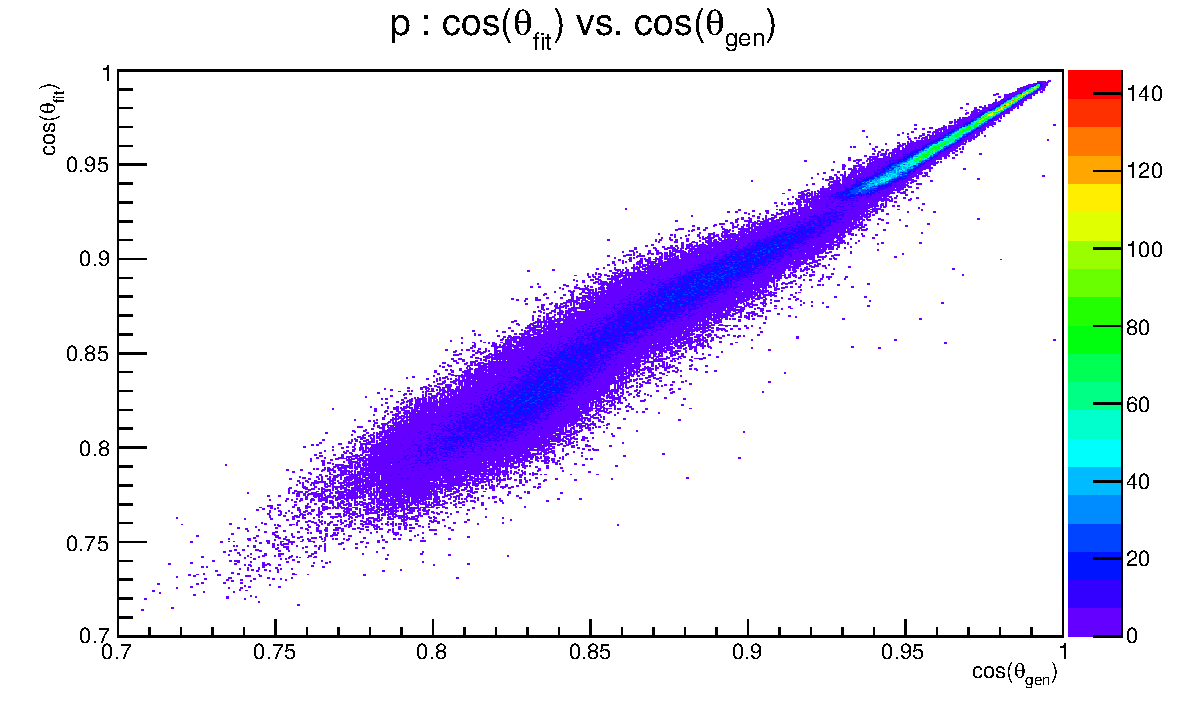
\includegraphics[width=8cm]{Plots/MC/1/ThetaTheta1Proton.pdf}
		\captionsetup{labelformat=empty}
		\caption{cos($\theta_{fit})$ vs. cos($\theta_{gen}$) for all protons.}
	\end{figure}
\end{frame}

\begin{frame} {$\omega$: $\theta_{fit}$ vs. $\theta_{gen}$}

\begin{figure}
	
	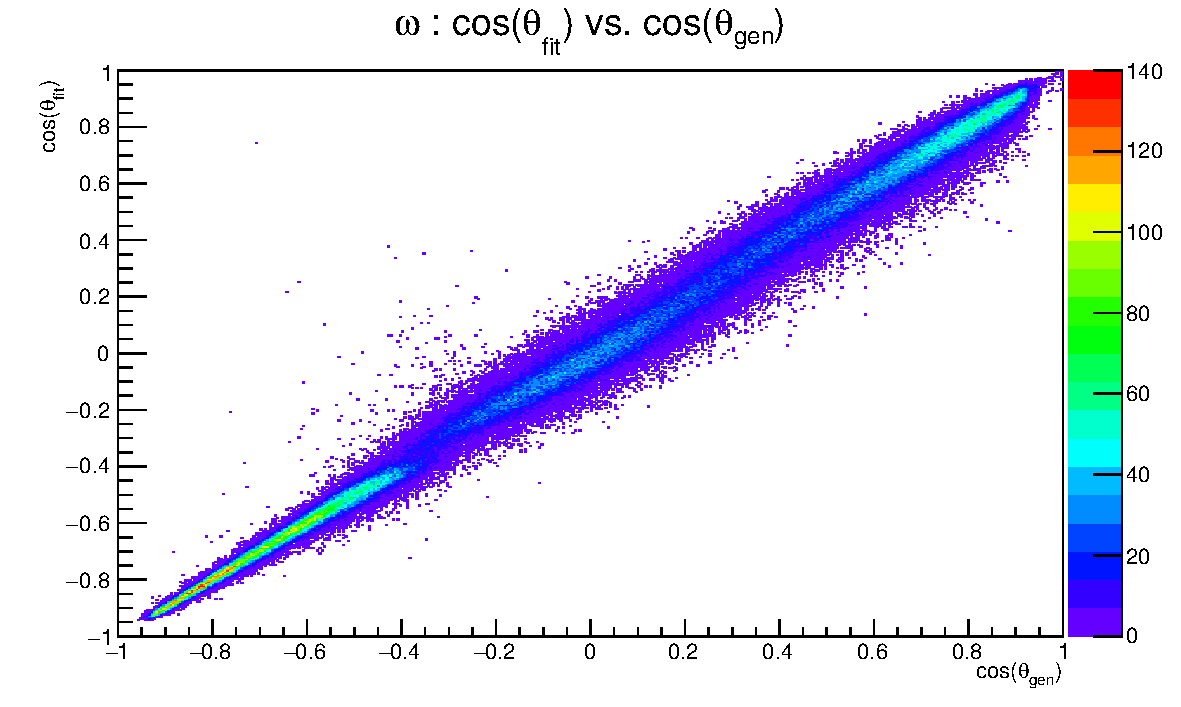
\includegraphics[width=8cm]{Plots/MC/1/ThetaTheta1Omega.pdf}
	\captionsetup{labelformat=empty}
	\caption{cos($\theta_{fit})$ vs. cos($\theta_{gen}$) for all $\omega$.}
	
\end{figure}

\end{frame}

%\begin{frame}{Conclusion}
	
%\end{frame}



\section{Unfolding}

\begin{frame}{Motivation}
	\begin{itemize}
		\item $\mu$ is the \textit{true} distribution given by nature
		\item detector effects are then described by the migration matrix \textit{R}. (inefficiencies, bias and smearing)
		\item This results in the distribution $\nu$. 
	\end{itemize}
	%\begin{equation*}
		\begin{center}
$		\nu_i = \sum_{j=1}^{M} R_{ij} \mu_j$  
		\end{center}
	%\end{equation*}
	
	\begin{itemize}		
		\item With infinite statistics, it would be possible to recover the original distribution by inverting the migration matrix
		
	\end{itemize}

\begin{equation*}
	\mu = R^{-1} \nu
\end{equation*}
%Unfortunately there are statistical fluctuations between bins and since R washes out statistical fluctuations R^-1 cannpt distinguish between wildly fluctuating and smoot distributions.

\begin{itemize}
	\item Use numerical methods to invert the migration matrix
\end{itemize}


\end{frame}

\begin{frame}{Unfold Example}




	\begin{figure}
		\vspace{0cm} 
		
		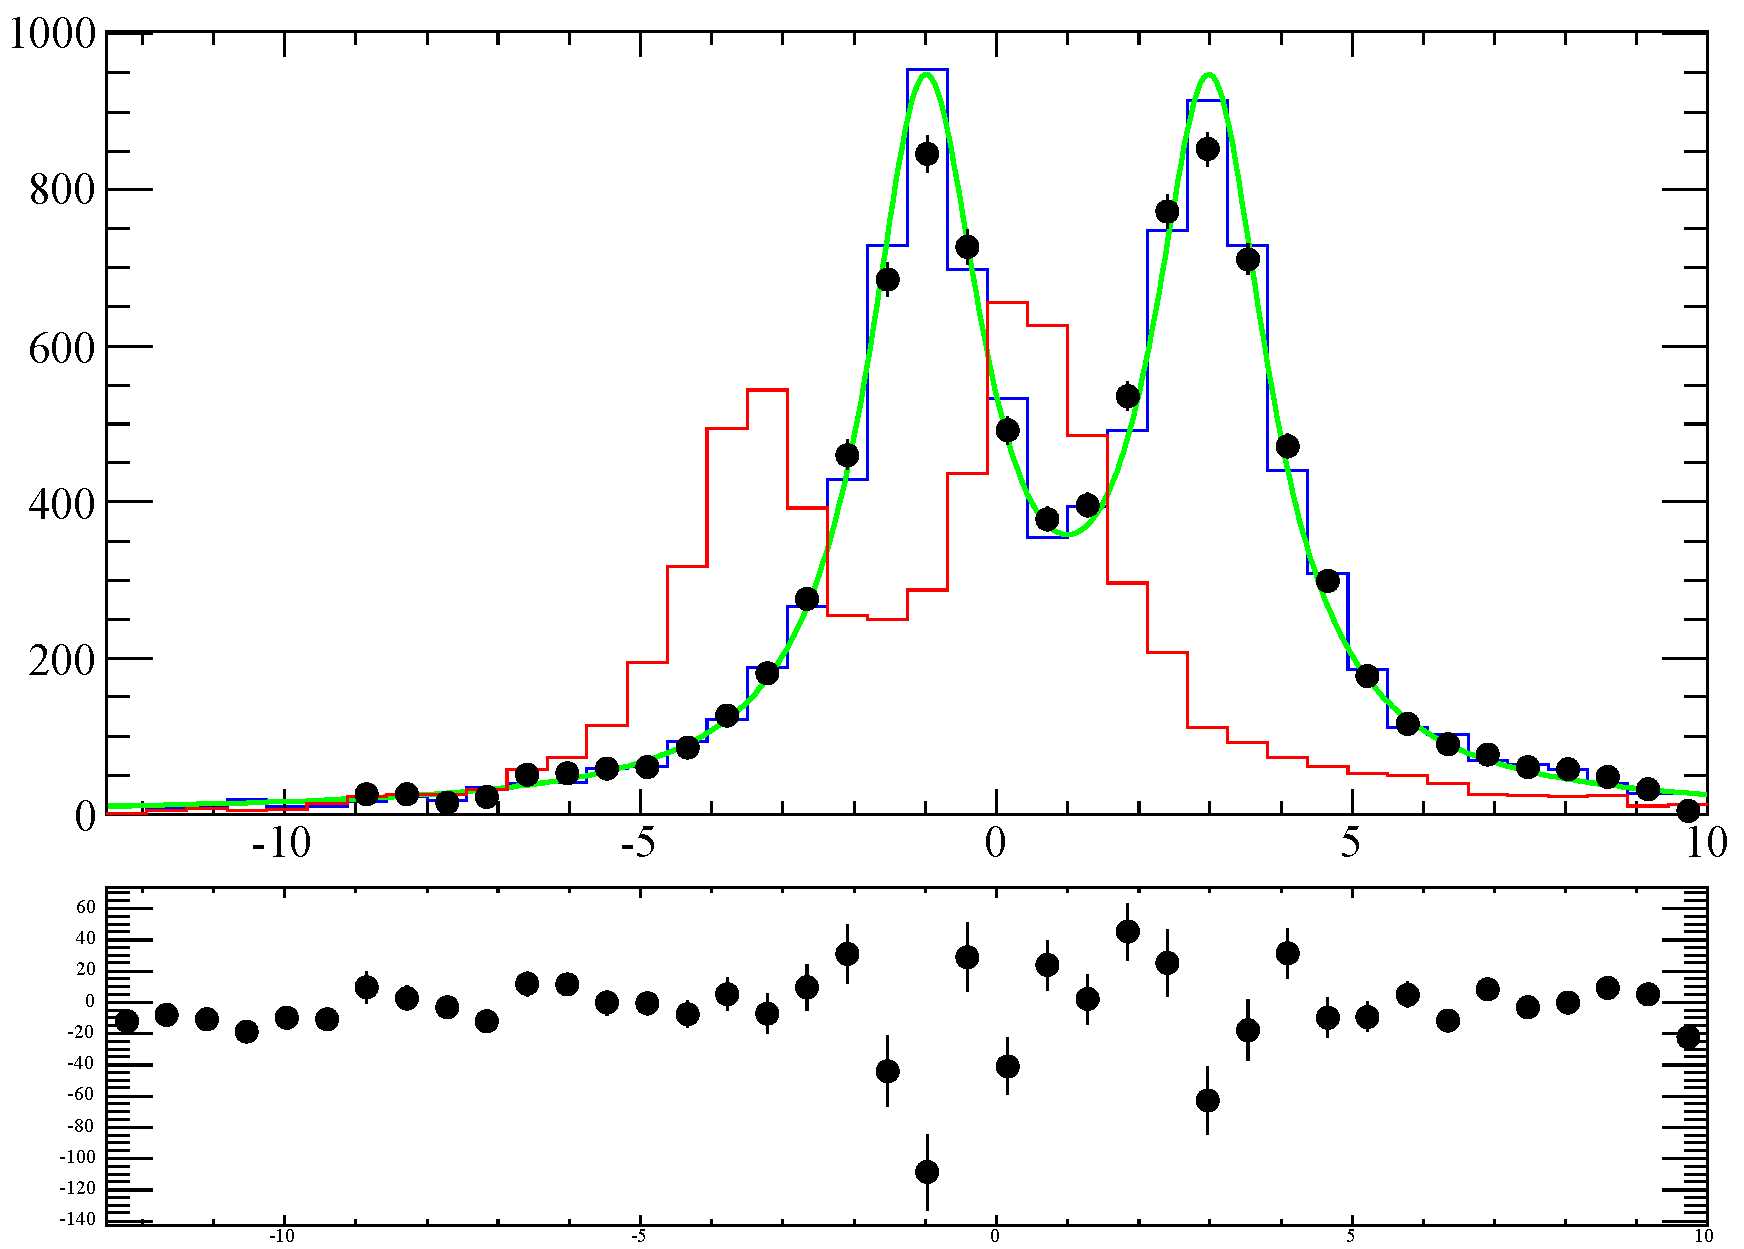
\includegraphics[width=8.0cm]{Plots/Tim}
		\captionsetup{labelformat=empty}
		\caption{Example for Unfolding. Blue is true distribution. Red is measured distribution. Black Dots are the unfolded distribution. Green is the fit of the unfolded distribution}
	\end{figure}
	
	\note{In region of $cos \theta(\omega)_{gen} \approx -0.35$, see broader distribution of
		$cos \theta(\omega)_{fit}$ -->  simple 1D efficiency correction may not
		work well enough}
	

	
	
\end{frame}





\iffalse


\begin{frame}{What is Unfolding?} 
\begin{itemize} 
		\item  Using MC we can train the unfolding algorithm
		\item Create a 2D-Hist with $ \textrm{cos}(\theta_{\omega}) $ of all generated and all reconstructed $\omega$ ($\omega$ which are generated but not reconstructed are label \textit{miss})
		\item Then we can solve for $\mu$ iteratively	
	\end{itemize}

\end{frame}


\begin{frame}{Example with Gaussian}
	
\begin{figure}
	\includegraphics<1>[width=8cm]{Plots/truth}

	\includegraphics<2>[width=8cm]{Plots/meas_truth}
	\includegraphics<3>[width=8cm]{Plots/folded}
	\captionsetup{labelformat=empty}
	\caption{Example for a working Unfolding Algorithm}
\end{figure}
	
	
\end{frame}




\begin{frame}{Folded}
	\begin{figure}
		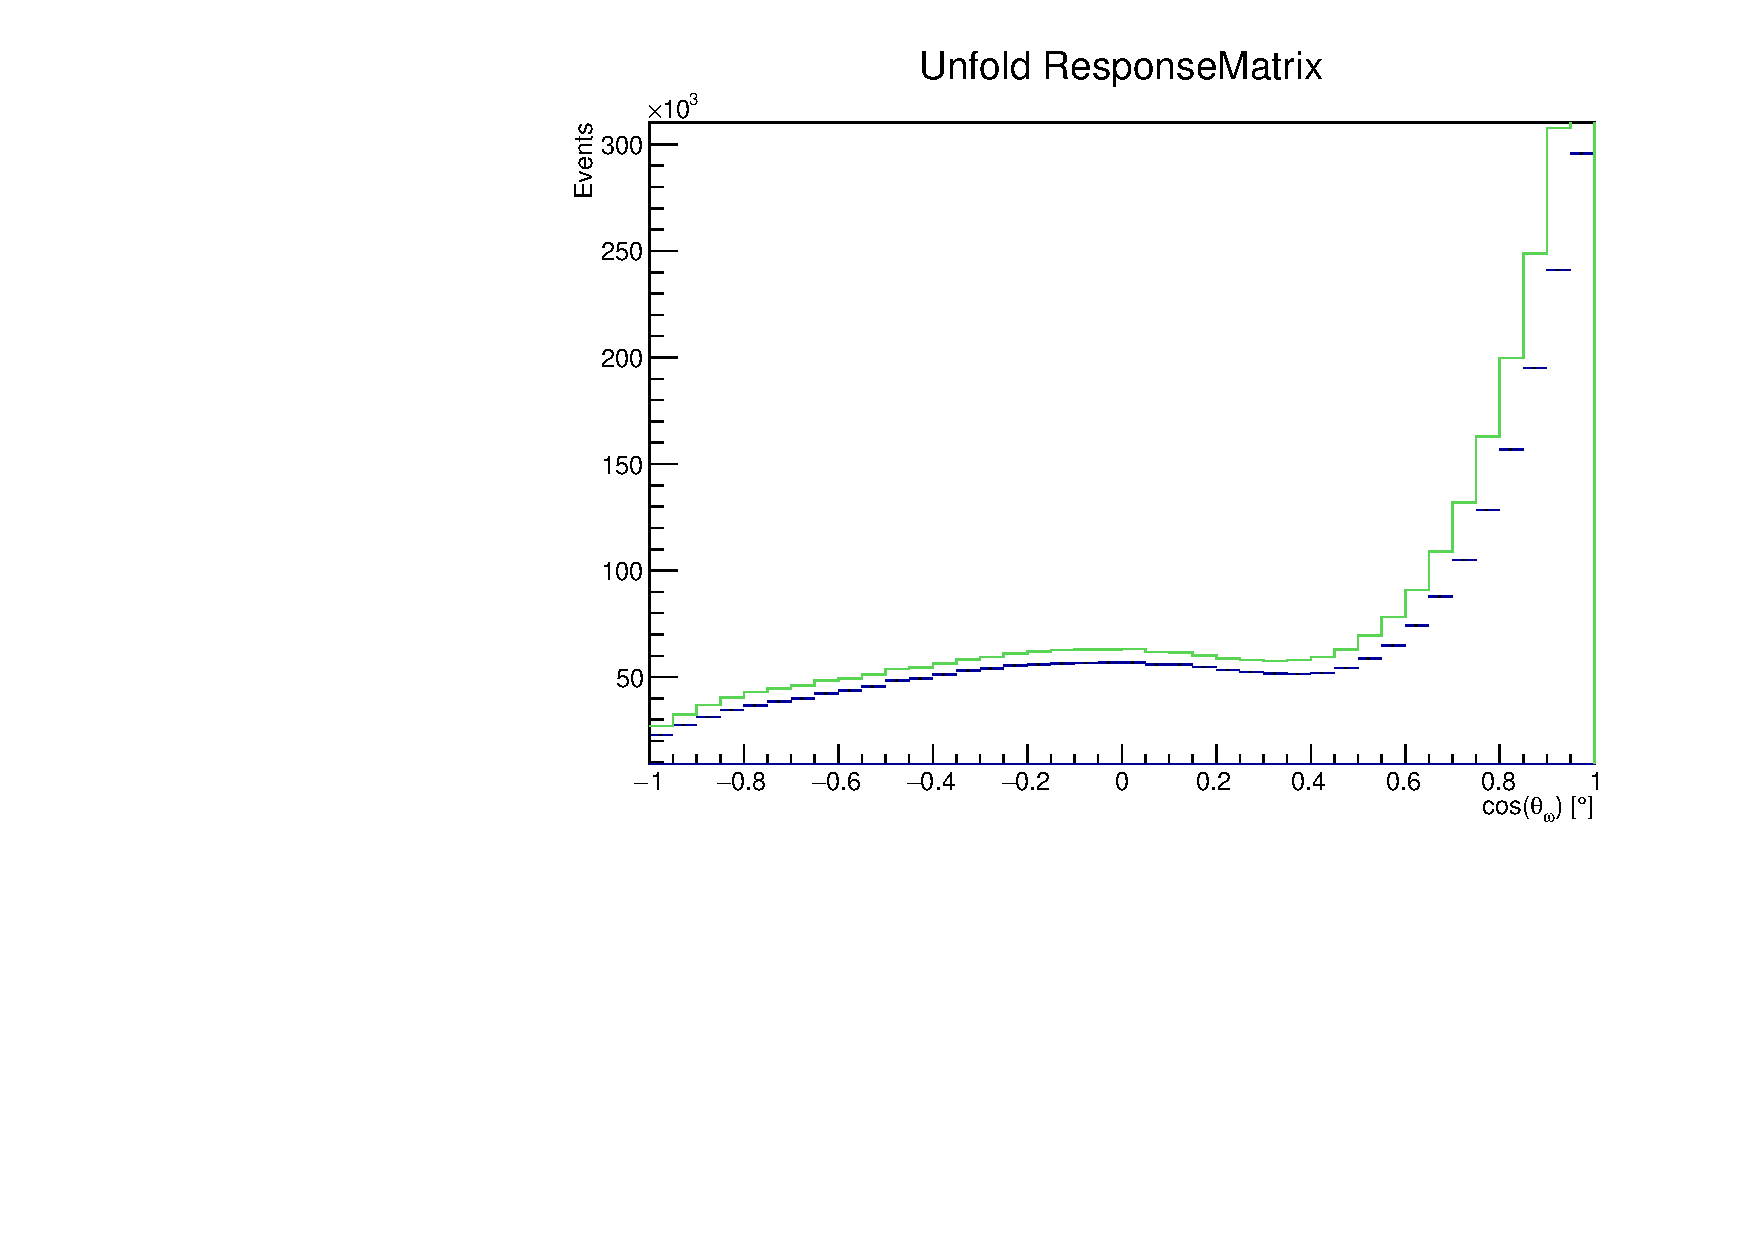
\includegraphics[width=8cm]{Plots/WholeUnfold35.pdf}
		\captionsetup{labelformat=empty}
		\caption{Folded; same cuts}
	\end{figure}
\end{frame}

\begin{frame}{Flat $\omega$}
	\begin{figure}
		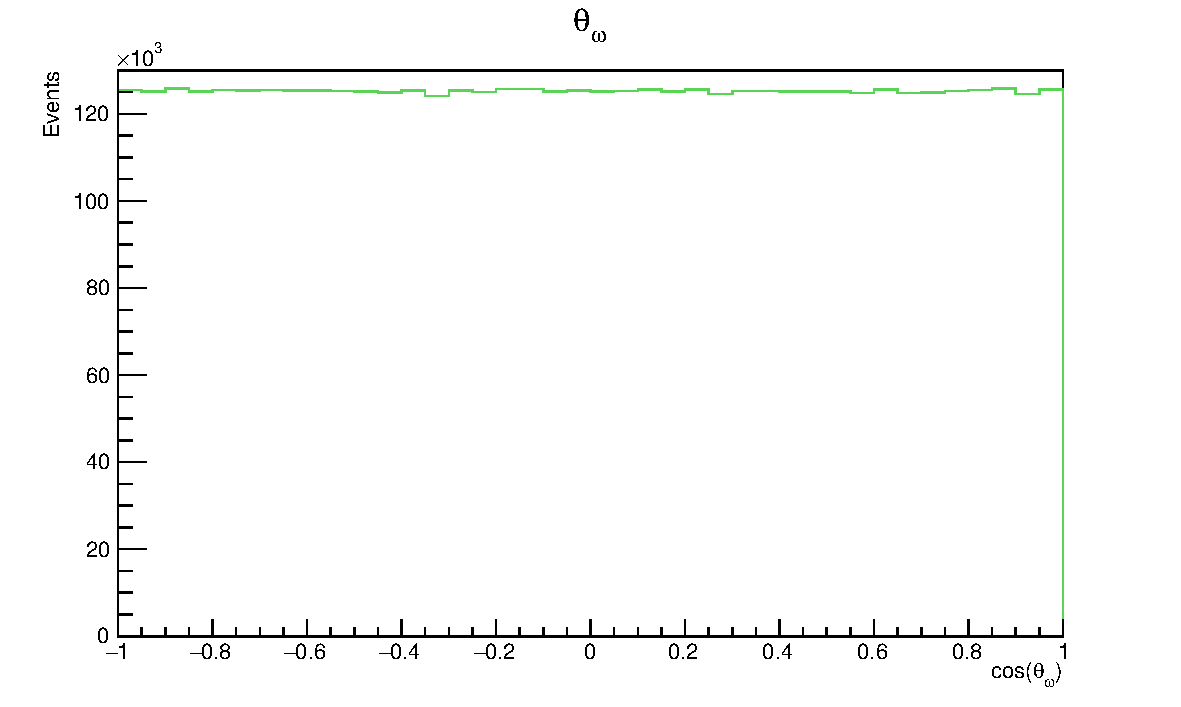
\includegraphics[width=8cm]{Plots/OmegaFlat.pdf}
		\captionsetup{labelformat=empty}
		\caption{Distribution of the $\omega$ in center of mass frame}
	\end{figure}
\end{frame}





\begin{frame}{Flat $\omega$; Folded MC Data}
	
	
	\begin{figure}
		
		
		
		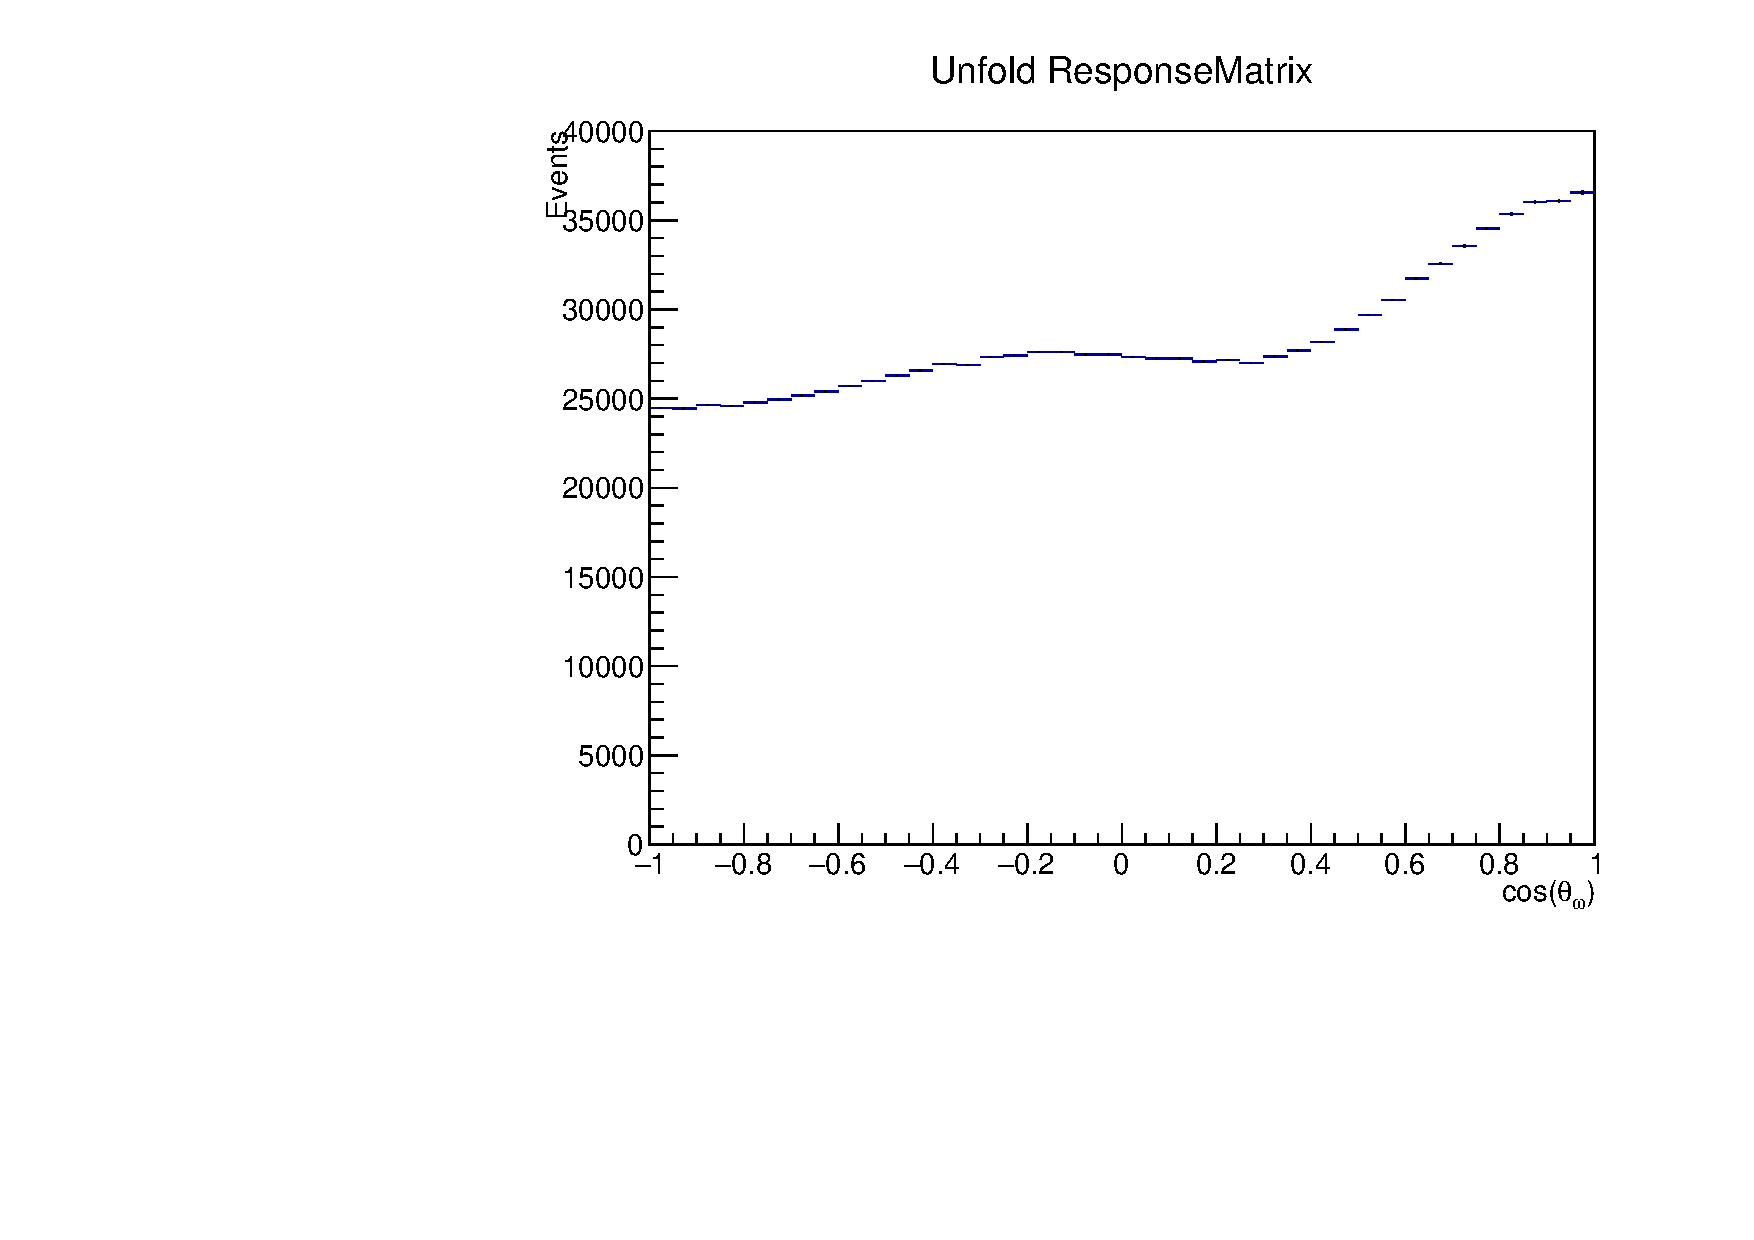
\includegraphics[width=8cm]{Plots/FlatMC.pdf}\\
		\captionsetup{labelformat=empty}
		\caption{Flat $\omega$ was used. MC fitted data were unfolded.}
	\end{figure}
\end{frame}


\fi


\begin{frame}{Flat $\omega$; Folded MC Data}



	
	\begin{textblock*}{6.5cm}(0.6cm,1cm)
		
		\begin{figure} 
		
		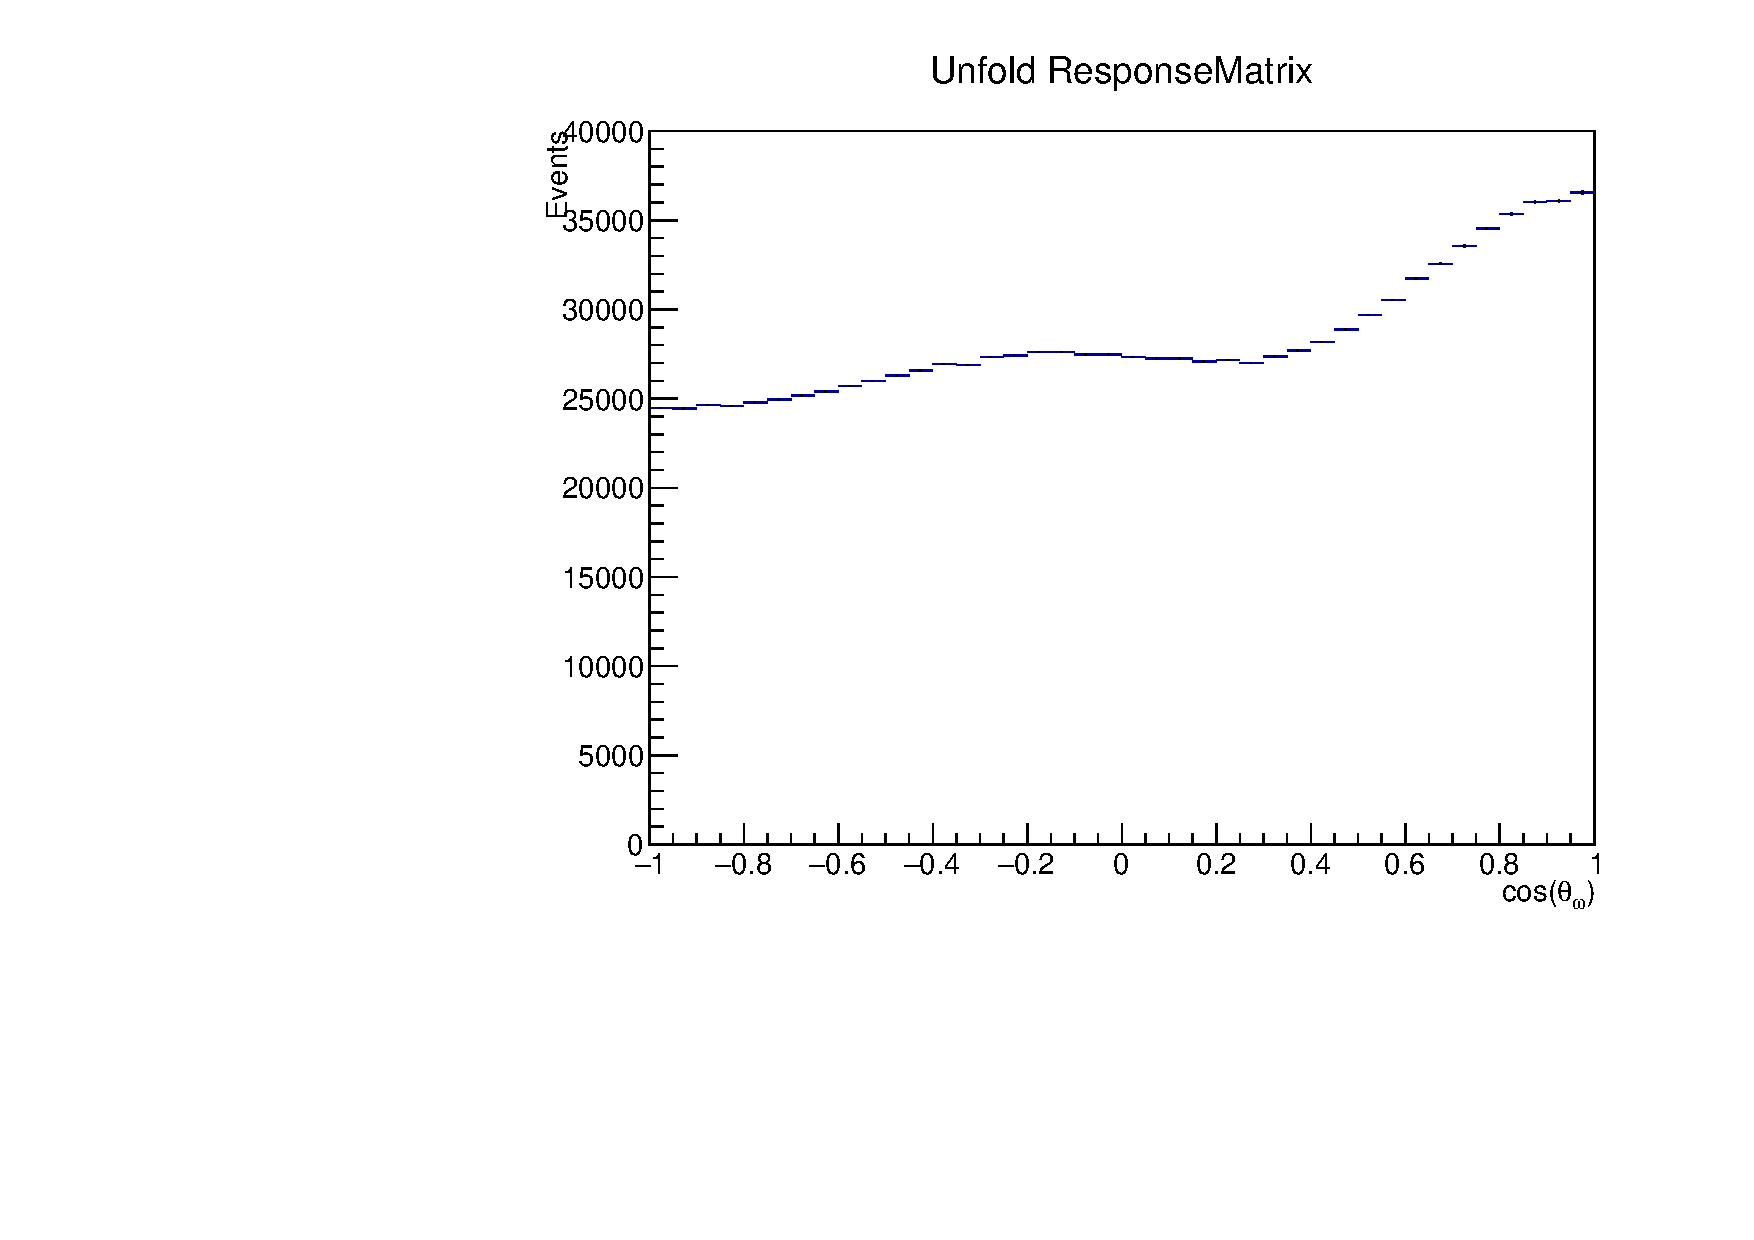
\includegraphics[width=8cm]{Plots/FlatMC.pdf}
		\captionsetup{labelformat=empty}
		\caption{Flat $\omega$ was used. MC fitted data were unfolded.}
\end{figure}	
\end{textblock*}

\begin{textblock*}{4.5cm}(8.05cm,1.7cm)
	\begin{itemize}
		
		\item $\omega$ are generated with a flat phase space
		\item A migration matrix is calculated 
		\item This migration matrix is than used to unfold realistic MC 
		\item Unfortunately, the unfolded cross section does not have the desired shape
		
		$\rightarrow$ Unfolding was unsuccessful
	\end{itemize}
\end{textblock*}


\end{frame}





\begin{frame}{Conclusion}
	\begin{itemize}
		\item Drop in the measured cross section at $\textrm{cos}(\theta_{\omega}) \approx -0.35$ is caused by a drop in the efficiency at that region
		\item Inefficiency is caused by the protons hitting the edge of the CB
		
		$\rightarrow$ They are not reconstructed properly
		\item There are differences between MC and Data
		\item The differences are too big to make the Unfolding work
		
	\end{itemize}
	
	
\end{frame}

\appendix


% And your backup slides here

\begin{frame}{Backup}

\begin{figure}
	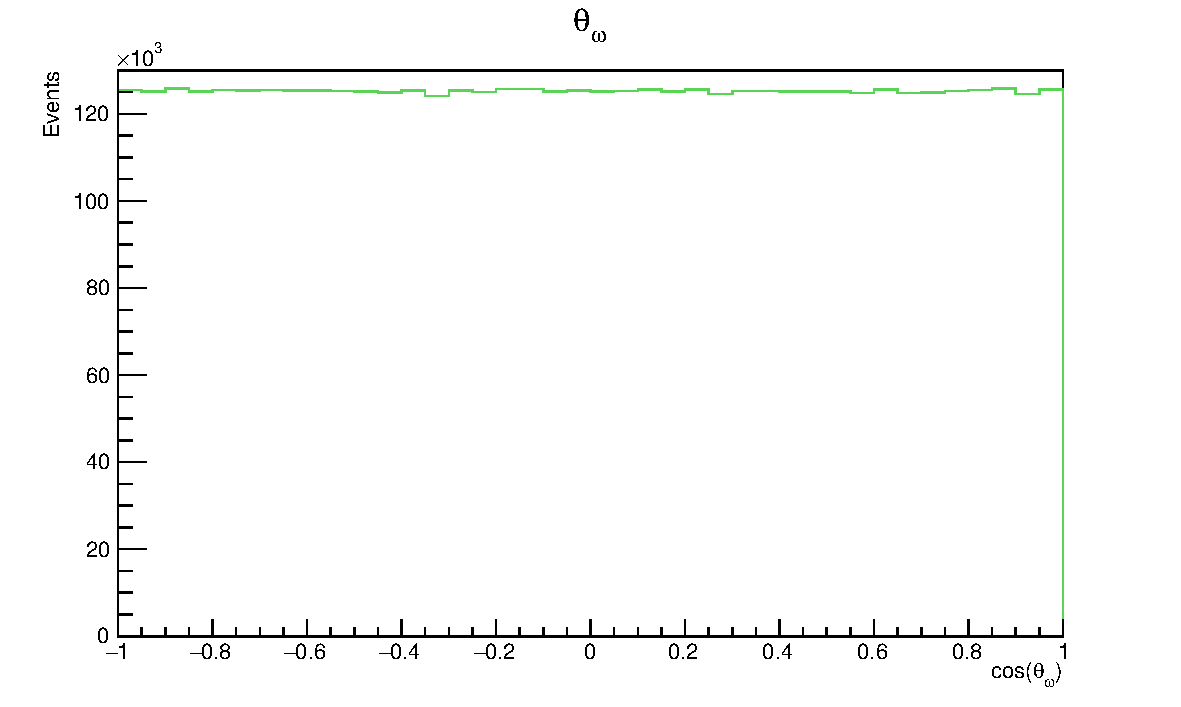
\includegraphics[width=8cm]{Plots/OmegaFlat}
	\captionsetup{labelformat=empty}
	\caption{Flat generated $\omega$}
\end{figure}



\end{frame}



\end{document}
